\documentclass[../main.tex]{subfiles}
\graphicspath{{\subfix{../images/}}}

\begin{document}

\begin{newrequirements}
    \textbf{Note that this section is a substantial 
    portion of the grade for your final 
    report and will require a significant 
    amount of effort.}

    \begin{todolist}
    \item describe in detail the tests you have 
        conducted to verify that your prototype 
        satisfies the desired functional 
        requirements while meeting the design 
        constraints. For example, if you used 
        Use Cases to describe your non-
        functional requirements, then for each 
        use case you should write a test case, 
        run it and report the testing results
        (the key test cases can be added as an 
        Appendix). Functional testing will 
        allow you to find defects then fix them 
        and also identify possible 
        improvements.  You need to have a 
        comprehensive set of tests that 
        verifies correct functionality of every 
        component of your system. 

    \item verify and provide evidence through 
        testing that your solution solved the 
        stated problem and satisfied the 
        requirement specifications and design 
        constraints, documented in Section 3.2 
        of the interim report. If not, explain 
        what is lacking and identify possible 
        improvements 

    \item This section must present sufficient 
        evidence and clear discussion that your 
        design and prototype met/did-not-meet 
        all of the identified technical and 
        practical constraints documented in 
        Section 3.2. You may use a summary 
        table to elaborate these points. The 
        table columns could contain: 

    \begin{todolist}
    \item Brief description of the constraints 

    \item Explanation of the testing steps taken 
        to evaluate if the constraint was met 
        or not. 

    \item Measurements data that prove your 
        system met/did-not-meet the constraint. 
        Also compare measured data against 
        expected values, then include a \%error 
        as (actual – expected)/expected*100\%, 
        and use only three digits of precision. 
        In case a constraint is not met, then 
        explain the reason for that. 
    \end{todolist}

    \item For further details and examples refer 
        to the document titled ‘Examples of how 
        to address and verify some of the 
        design constraints’ posted on the 
        Senior Projects website. 
         
    \item Describe in detail the tests performed 
        on the individual subsystems of your 
        project.  Discuss how you tested each 
        subsystem and what the results of each 
        test were. 

    \item In addition, do not forget to include: 

    \begin{todolist}
    \item If you have a GUI of some type, you 
        need a screen shot of it. 

    \item If you have a physical display of some 
        type (LEDs, LCDs, etc.), you need a 
        photograph of the display showing 
        typical operation. 

    \item For any interfaces of your hardware 
        components – USB, I2C, SPI, RS232, 
        parallel interfaces, or A/D inputs – 
        you may show oscilloscope pictures that 
        demonstrate a sample data transfer of 
        this interface and the typical 
        voltage/frequency ranges. 
    \end{todolist}

    \item You should present the test results, 
        with appropriate level of details in 
        addition to accuracy and completeness, 
        using tables, graphs, diagrams, screen 
        shots etc. Additionally, discuss these 
        results and explain whether the 
        prototype has achieved the 
        requirements. If not state what is 
        lacking or still need improvement then 
        explain the reason for that. There will 
        probably be multiple subsections under 
        this section to describe each system 
        test and its result. 

    \end{todolist}
\end{newrequirements}
In this section we will list all the conducted unit 
testing and integration testing and its results.
\begin{table}[H]
    \centering
    \caption{Summary of the unit testing}
    \label{tab:testing-summary}
    \newcolumntype{b}{l}
    \newcolumntype{s}{>{\hsize=.6\hsize}X}
    \begin{tabularx}{\textwidth}{bssss}
        \toprule
        \textit{Constraint} 
            & \textit{Testing procedure} 
                & \textit{Result}
        & \textit{Measurement data} 
            & \textit{Error (\%)} \\

        \midrule
        
        
        Power supply    & Test the capacity and the health of the batteries 
        and check if they produce power the same as in the specifications label or not. 
        & Met, but the batteries' life cycle will be less when time goes by,so it should be replaced after a particular time.
            & raspberry pi battery : \SI{1.9}{hours}, \anafi drone battery :\SI{2.8}{hours}
        &  raspberry pi battery error : 52.5\% , \anafi drone battery error : -3.7\%\\
        
        Flying duration & when the batteries if full
        measure the drone flying duration at different actions such as hovering, moving. 
        & Met
        & hovering: \SI{14.78}{minutes}, moving:  \SI{13.58}{minutes}
        & hovering flying duration error :1.47\% , moving flying duration error :9.477\% \\
        
         Response & Send the command to the drone and see the consumed time to start executing and should be below 1 second as in the technical design constraints.
        & Met
        & \SI{0.1511}{second}
        & 0 \\
        
         Payload & Test the maximum payload by increasing the load gradually 
         until you find the weight that the drone cannot handle. 
        & Met
        & \SI{193}{gram}
        & 0 \\
        
        Economic & the costs didn't exceed the expected value 
        & Met
        & \qar{3800}
        & 0\% \\

        \bottomrule		
    \end{tabularx}
\end{table}

%% Each subsection corresponds to a test.
%% Title the subsection based on the functional requirement OR
%% the design constraint being tested.

% HARDWARE
\subsection{Unit testing}
In this section, we will discuss all the conducted tests 
and challenges regards the design constraints. 

\subsubsection{Connecting to the drone}

We have connected the
Raspberry Pi to the drone using built-in WiFi
to allow the Raspberry to send/receive control and status 
instructions to the drone. 
For connecting Raspberry Pi to the laptop, 
we used the external WiFi adapter and turned 
on the hotspot feature to create an access point.
This made the process so convenient because 
once the Raspberry Pi boots up, it turns on the 
access point, and the user can connect to it 
easily and execute scripts using \textsc{ssh} 
protocol or open the web app user interface 
at www.aireye.com:8000. We executed the takeoff 
and move forward scripts and it worked successfully.
This way, we confirmed that we can connect to the drone and can control it effectively.

\subsubsection{Command-Control system maximum communication distance}

In this test we wanted to validate the maximum communication range that
the command and control system and the raspberry pi can communicate
and share live video feed. We fixed the command and control system and moved
the drone away from it, then for every 3 meters, we have measured the Signal-to-noise ratio (SNR).
We have repeated this experiment three times to get the average maximum range.
From the results shown in ~\ref{fig:snr-vs-distance}, after 117 meters 
the command and control system disconnects from the Raspberry Pi
and the video stream stops. Disconnecting is not a major issue
since once the Raspberry Pi receives the start mission commands, its 
and it will autonomously finish the mission and record the video needed
and once the connection is back users can continue control or interrupt the mission
at anytime.
 
\begin{figure}[!t]
	\centering
	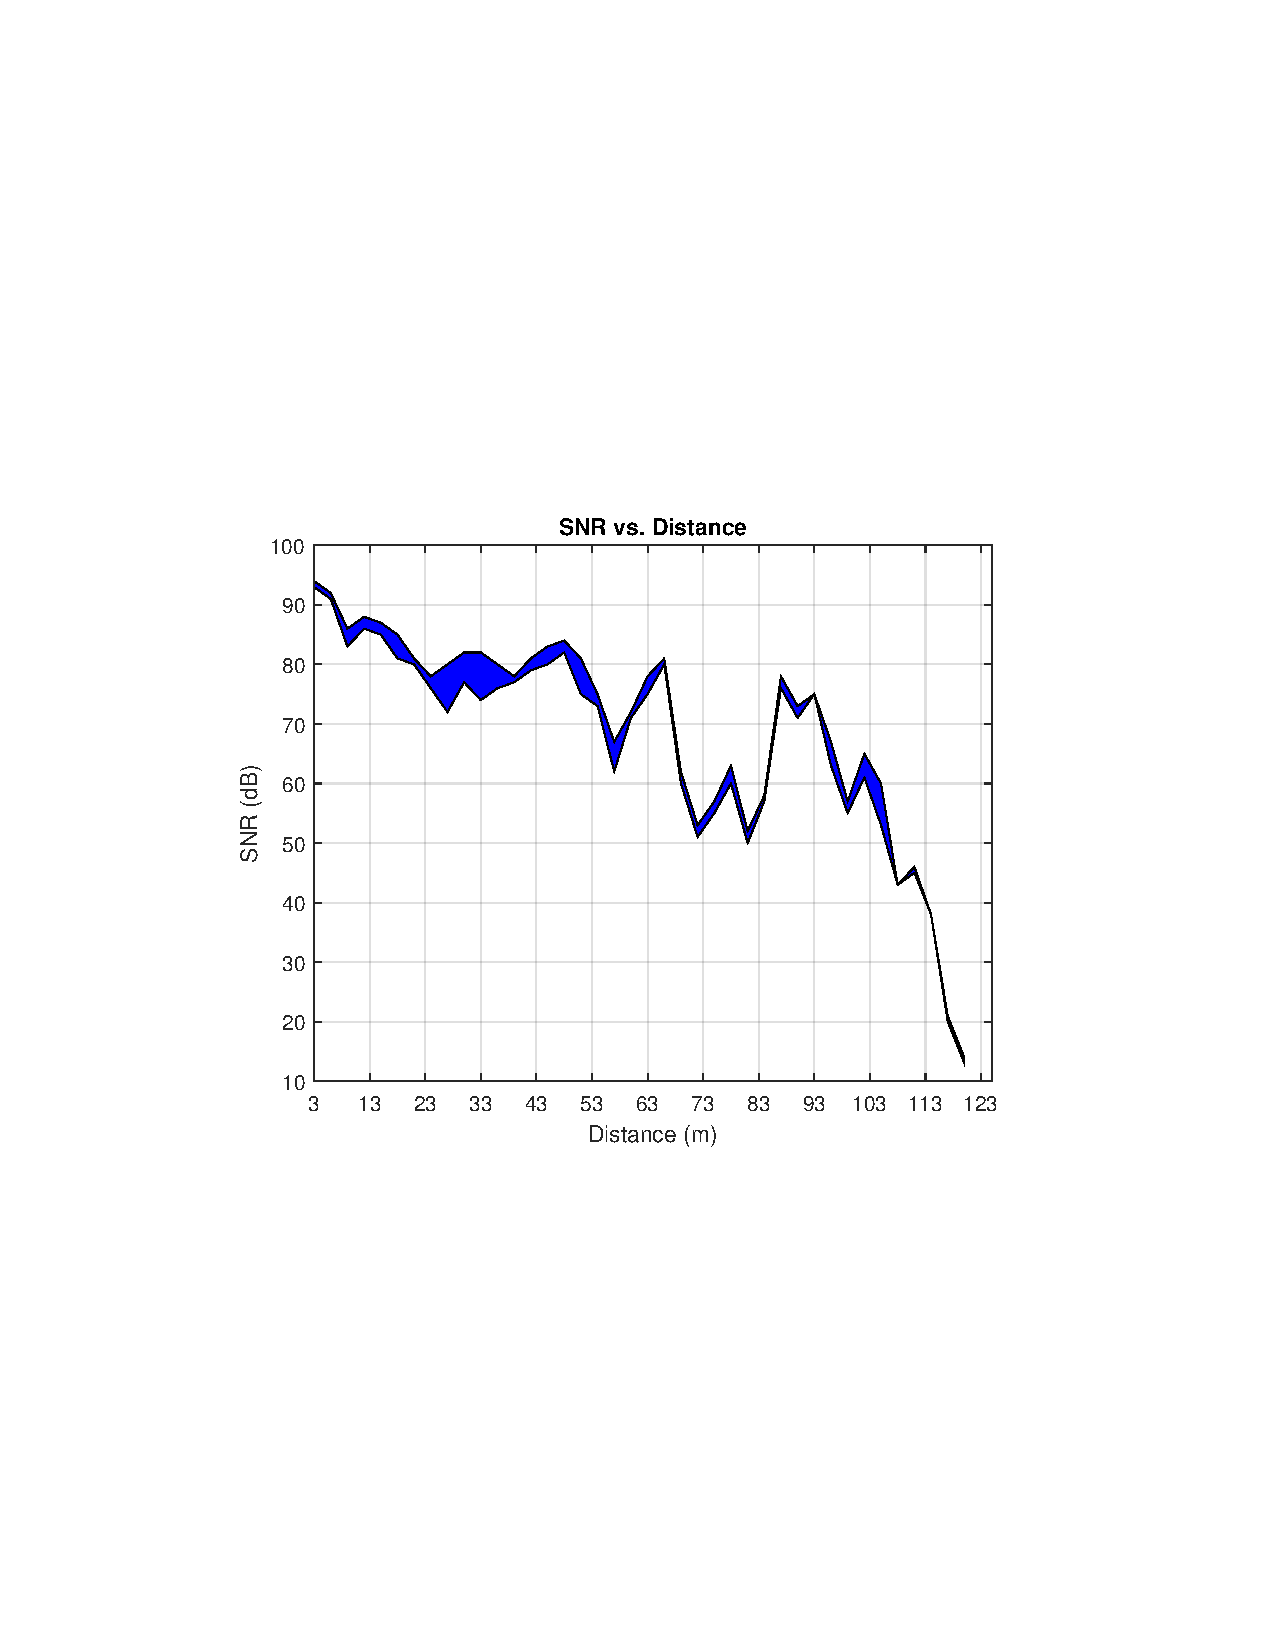
\includegraphics[width=5in]{snr}
	\caption{Average SNR vs Distance}
	\label{fig:snr-vs-distance}
\end{figure}

\subsubsection{Flying duration \& Batteries}

As shown in Fig.~\ref{fig:time-comparison} we have 
conducted time comparison experiments for both drone's
battery (2700mAh) and the Raspberry Pi battery (4000mAh) 
using different actions such as idle, hovering, 
moving forward, and moving backward. We repeated 
the same actions without video streaming so that 
we can see its effect on power consumption. 
All the batteries were charged fully, and the timer 
script stops when the battery percent reaches zero. 

First, as we predicted 
the maximum time reached is when both the drone and 
the Raspberry Pi are in an idle state, in which both case both will 
be on the ground without moving any motors.
This action still consumes energy but with 
its stability, over time ~\cite{Abey18}. 
The next action is when the drone is hovering, and 
the Raspberry Pi is sending navigation control 
signals to the drone and receiving video frames 
that are streamed to a web graphical interface. 
When the drone hovers without streaming, it worked 
for 14.78 minutes, and when the camera is used for 
the stream which will add more power consumption to 
the drone battery; it worked for 14.2 minutes which 
is less than the hovering without stream. The final 
action is when the drone takes off and keep moving 
forward, backward, left, and right, and in this action 
more energy consumption is seen and that made the 
battery for the drone survives only for 13.58 minutes 
when the camera is off, and for 13.18 minutes 
when the camera and stream are on.

The main focus will be on the drone battery and every 
action energy. This is because the raspberry pi battery 
is not being highly affected by the actions. 
The next step is to derive the energy model for every 
action by using the distance and time. For the drone battery, 
we have 2700mAh which is 20.52Wh ~\cite{Par19}, 
we can get the drone energy by multiplying Wh by 3600 
so we will have a total of 73,872 Joules. When taking
hovering without stream as an example, the battery 
went from 100 percent to 0 in 14.78 minutes which is 
886.8 seconds. We can say that the hovering action takes approximately 73,872/886.8 = 83.30 Joules/sec. For moving action,
we also considered the distance , so we kept 
moving the drone one meter in each direction 
{forward, backward, left, right} and then calculate 
the total distance traveled. The drone repeated 
the moving action 11 times, so the total distance 
is 44 meters and the energy per second consumed 
is 73,872/814.8 = 90.66 Joules/sec but this energy 
per second is for the 44 meters, so we can get the 
energy per second for 1 meter by calculating 
90.66/44 = 2.06 Joules/s. 
In (\ref{eq:Energy-moving}) we can generalize an energy equation for moving action, which can be used in the simulation environment to train the RL model. Now the model will not just consider the time, but also the energy consumption.
We verified the flight duration constraint, and we can devise some 
realistic energy models, that can be fed in the simulation to do the comparisons. This will help the RL model to choose 
the best action depending on less energy consumption 
when both actions have the same probability. 

\begin{align}
	P = \frac{E(J)}{t(s)} 
	\label{eq:power}
\end{align}

\begin{align}
	E = 2.06t*d
	\label{eq:Energy-moving}
\end{align}

\begin{figure}[!t]
	\centering
	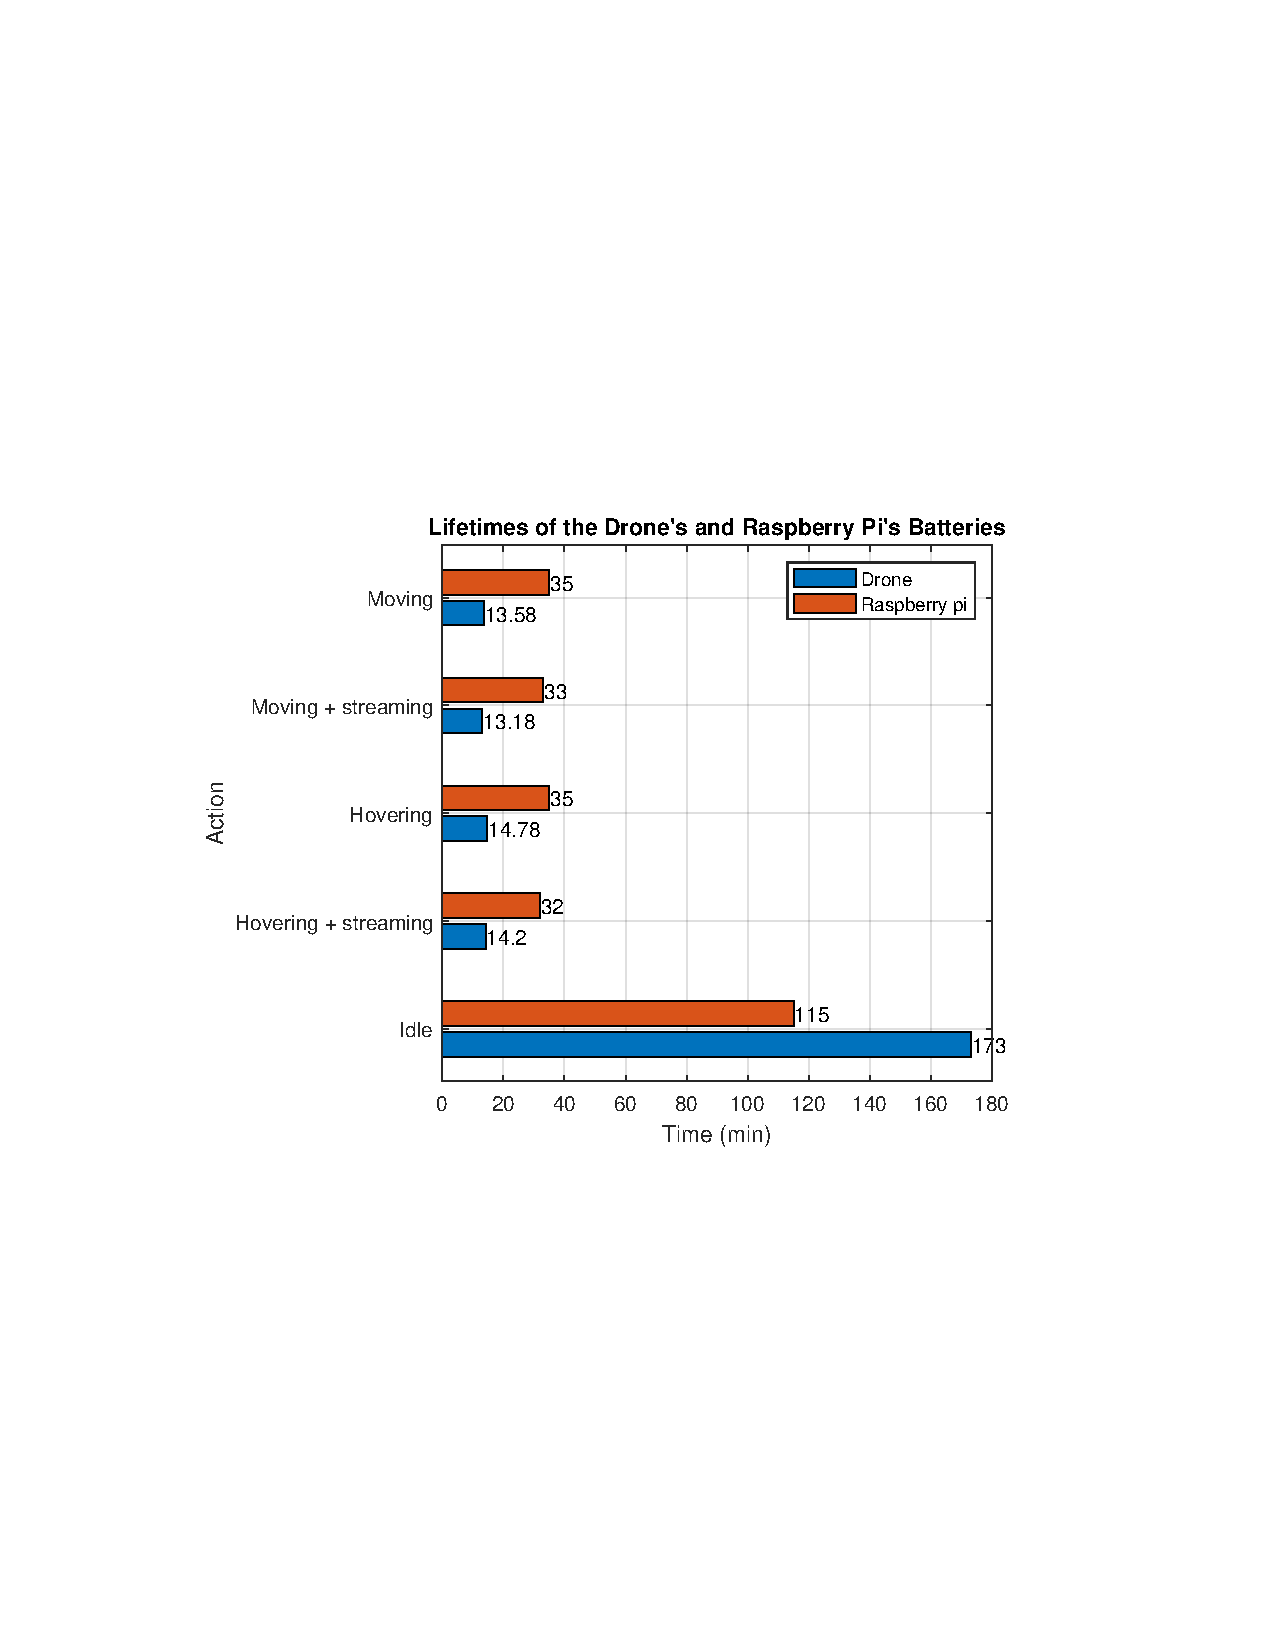
\includegraphics[width=5in]{battries-time}
	\caption{Battery's lifetime comparison.}
	\label{fig:time-comparison}
\end{figure}

\subsubsection{Response time}

We have done another experiment regarding the response time 
of the drone after sending a command to it from the Raspberry Pi. 
Calculating the response time was by starting a timer when 
sending the command and stopping it when the 
state of the drone changes. 
The experiment was done on simulation using Sphinx,
then we moved to the real world using the \anafi drone.
From \cref{tab:respone-time}, 
we can see that all the results are less than \SI{1}{second}
which satisfied our response time constraint.
Another point we can conclude from the table is that 
the response time of the real world is less than 
the simulation, and this is predictable since the simulation
depends on the \textsc{gpu} power and processing time. 

\begin{table}[H]
	\centering
	\caption{The average response time of the drone after sending a control command.}
	\label{tab:respone-time}
	\begin{tabularx}{0.7\textwidth}{ X c c }
		\toprule
		\textit{} & \textit{Simulation} & \textit{Real-world}\\ \midrule
		Motor ramping for takeoff (seconds)  & 0.3506 & 0.0323     \\
		Move while flying (seconds) & 0.7441  & 0.1511   \\
		\bottomrule
	\end{tabularx}
\end{table} 

\subsubsection{Payload}

As shown in \cref{fig:payload}
we attached \SI{190}{grams} of Raspberry Pi and Arduino boards
to see the effect on the performance, flight and
battery drain percentage. 
The drone has taken off  successfully, 
and the flight was normal, but we faced an expected 
battery drain that went from 
\SI{100}{\percent} to \SI{90}{\percent} in 
\SI{1.5}{minutes}. This is because the propeller motors will try to push 
their limits to take off the drone, which will consume more energy.
After adding payload to the drone at \SI{200}{grams}, the drone couldn't
takeoff and we now know the payload limit, which will be considered in the 
design constraints. In the actual design, as shown in 
\cref{fig:actual-total-weight} the total payload 
is \SI{193}{grams} which is less than the payload constraint.



\begin{figure}[H]
	\centering
	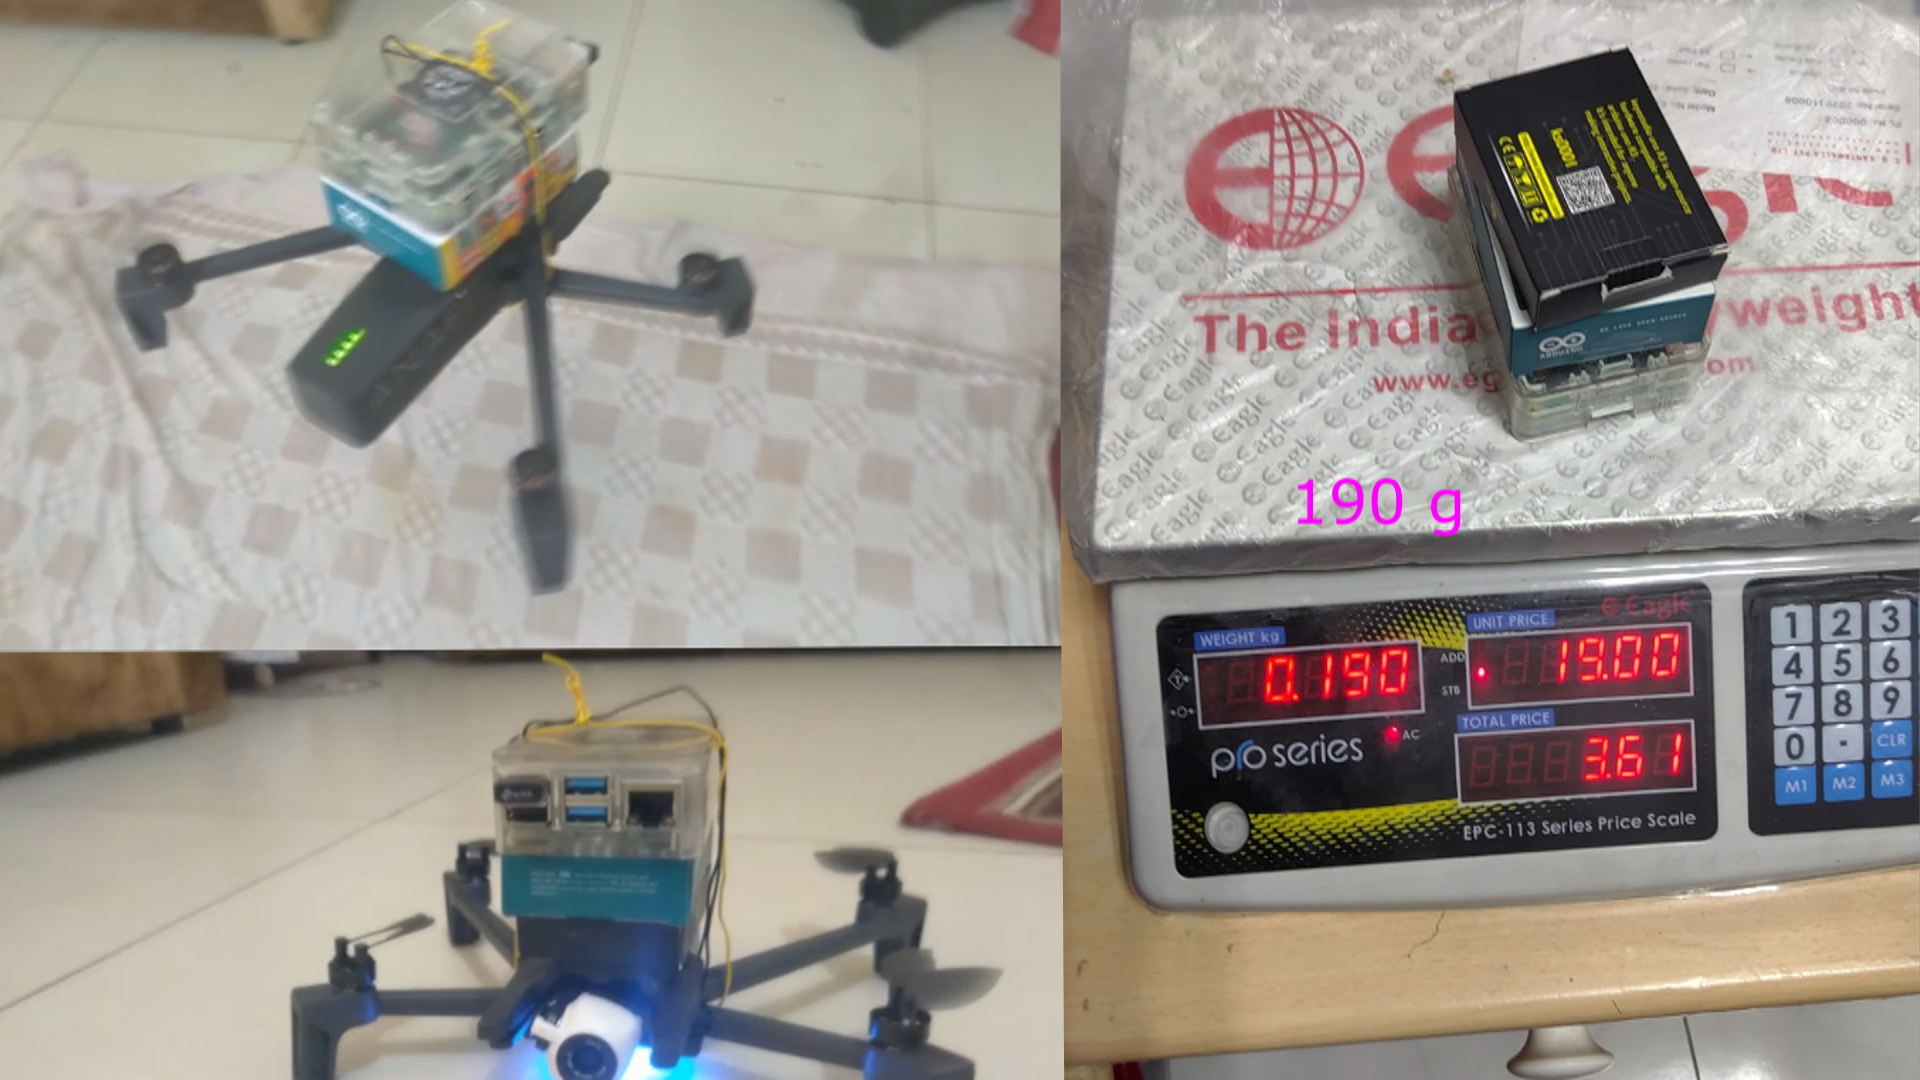
\includegraphics[width=0.6\textwidth]{payload.png}
	\caption{The total weight of test payload}
	\label{fig:payload}
\end{figure} 

\begin{figure}[H]
	\centering
	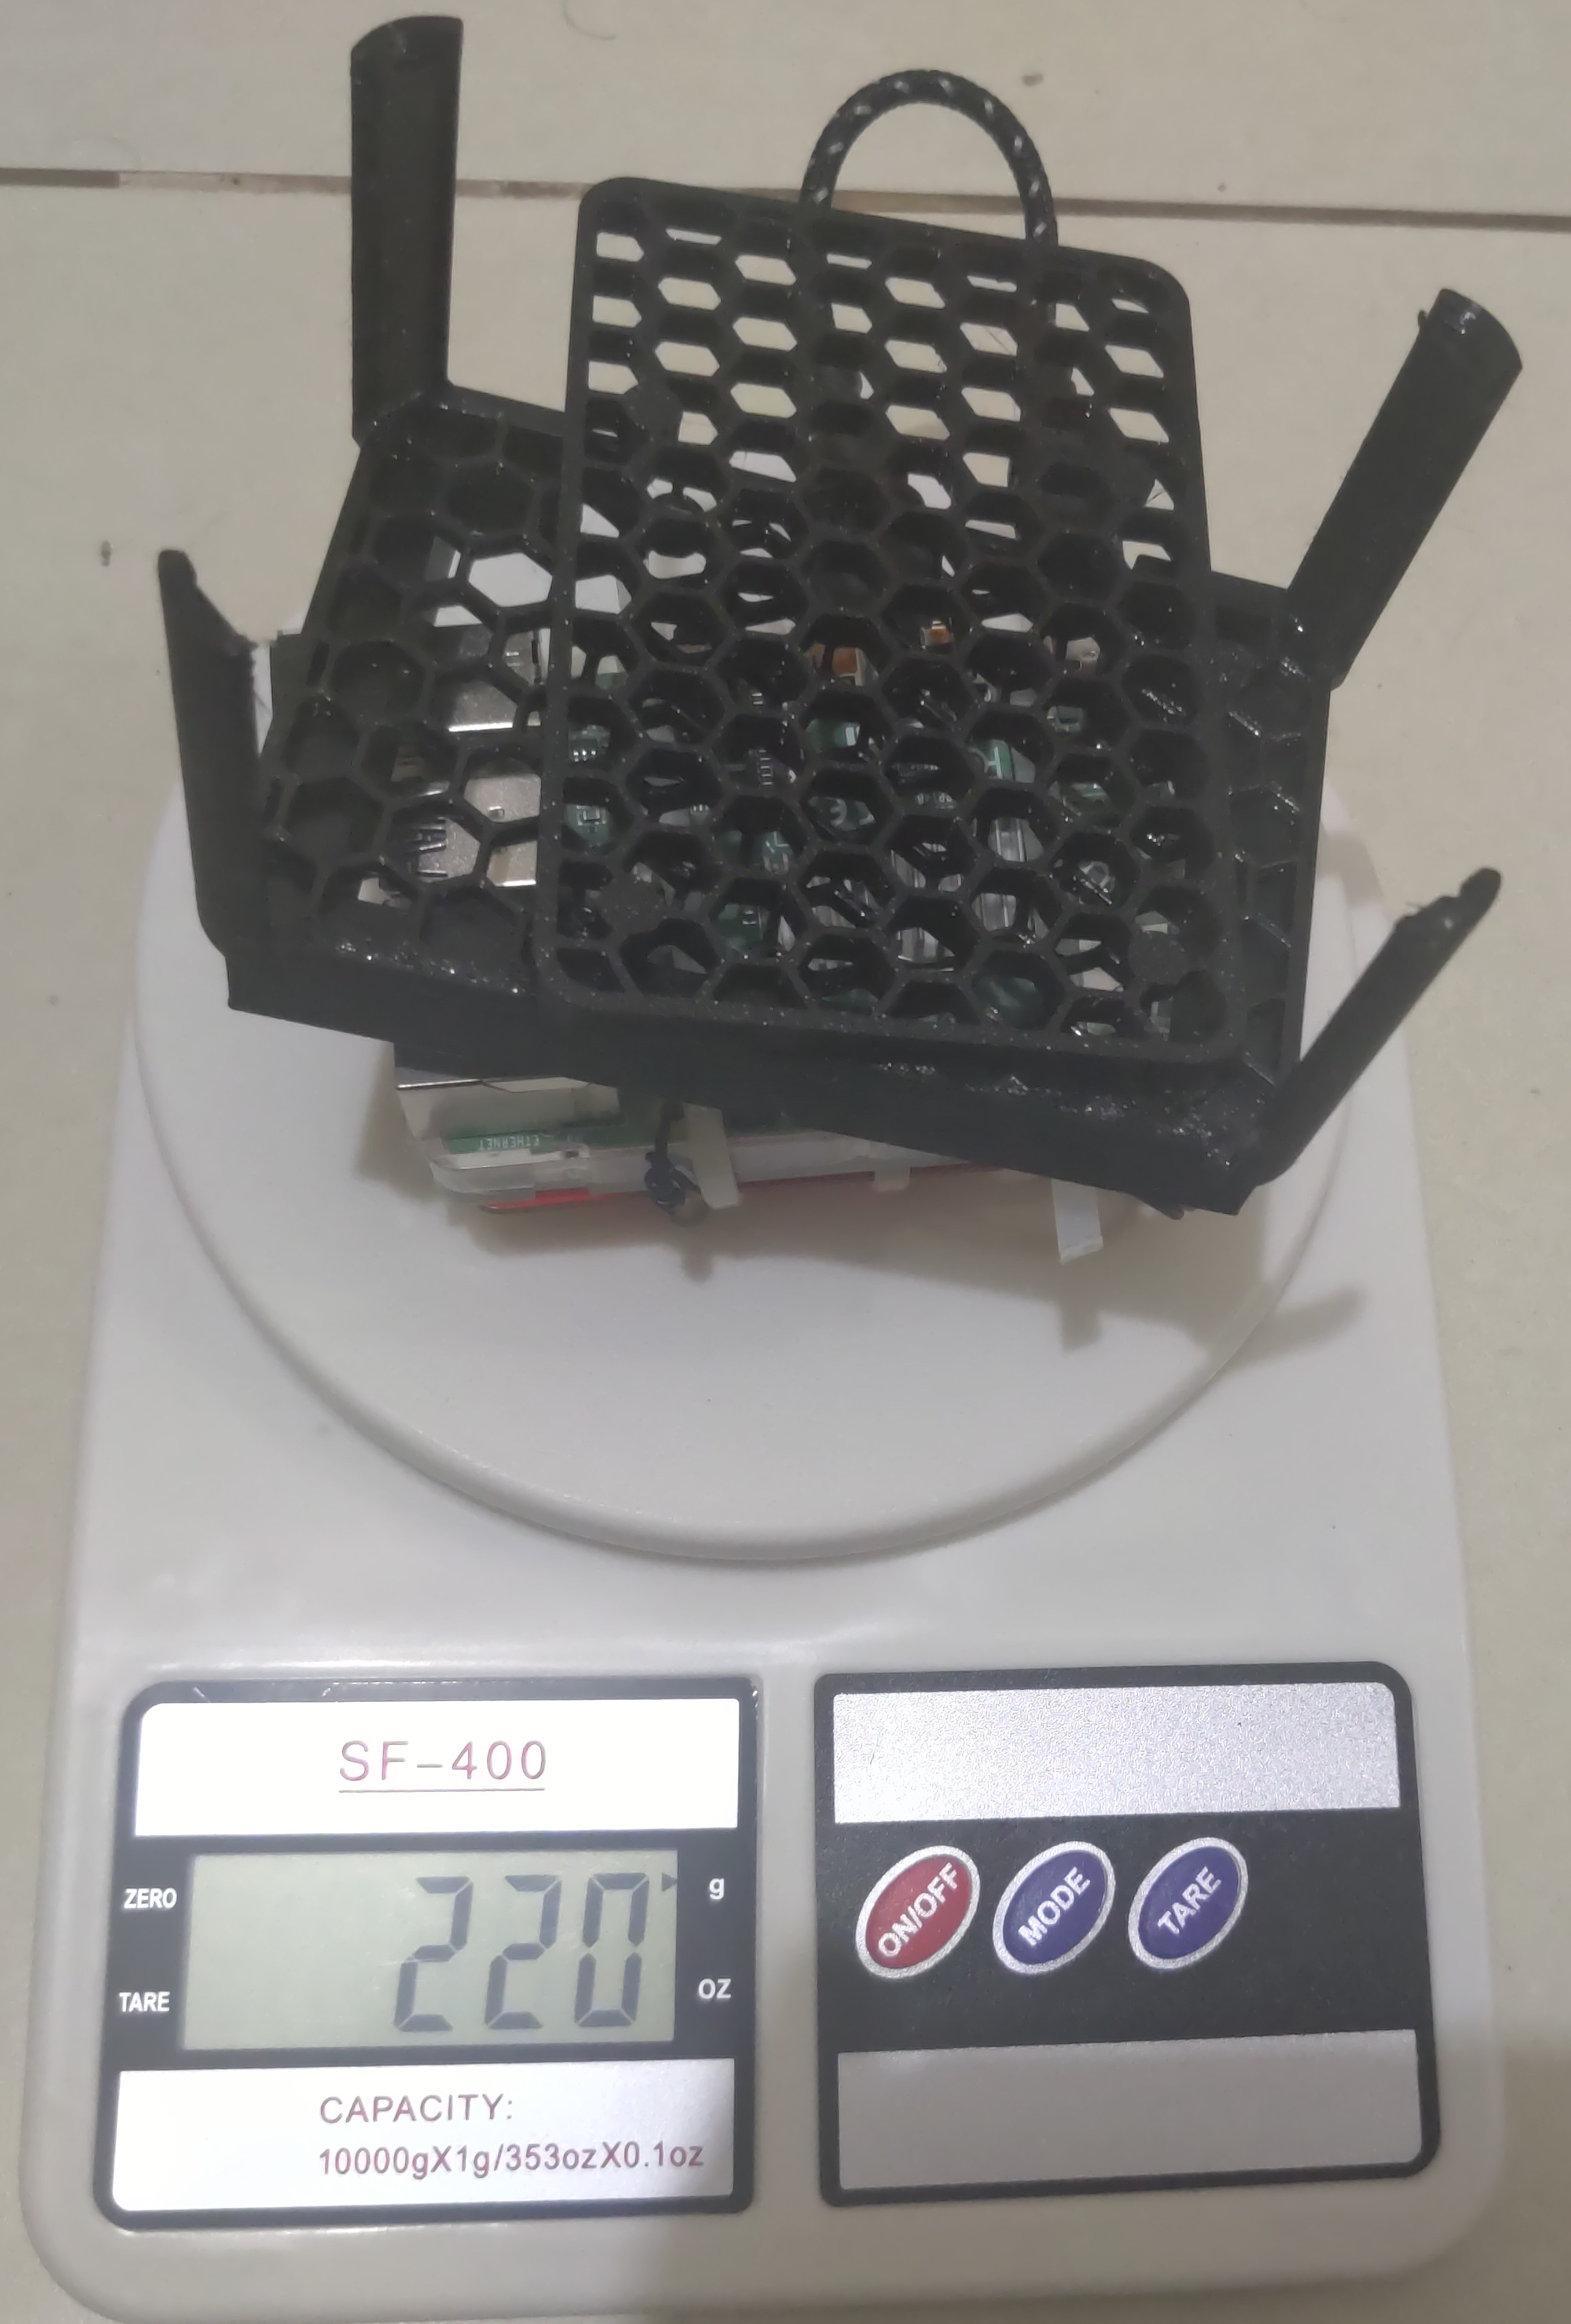
\includegraphics[width=0.4\textwidth]{totalweight.jpg}
	\caption{The total weight of actual payload}
	\label{fig:actual-total-weight}
\end{figure} 

\subsection{Integration testing}


% SOFTWARE
\subsection{Simulating the targets}

\lipsum[1]

\subsection{RL training}

\lipsum[1]

\subsection{RL model performance}

\lipsum[1]

\subsection{User interface}

\lipsum[1]


\end{document}
